\فصل{شبکه انباشت و شلیک}
\label{chap:integrate_and_fire}
در این نوشتار \cite{PhysRevLett.105.158104}  نویسندگان تلاش می‌کنند تا هم‌گامی را برای شبکه‌ی نورون‌های مهاری رصد کنند. این نورون‌ها به گونه‌ای باهم مرتبط هستند که تیزه زدن هر نورون منجر به مهار پتانسیل دیگر نورون‌ها می‌شود. تک‌تک نورون‌های این شبکه از تحول انباشت و شلیک تبعیت می‌کند. معادله تحول اختلاف پتانسیل هر کدام از نورون‌ها با محیط بیرونش از رابطه زیر داده می‌شود:
\begin{tcolorbox}
	\begin{align}
		\dot{v_i}=a_i - v_i - \frac{g}{N} \sum_{n|t_n<t} S_{i,l(n)} \delta(t - t_n - t_d) 
		\label{eq:potential_1}
	\end{align}
	
	\begin{enumerate}[-]
		\item
		$g$: 
		ضریب اتصال هر جفت نورون. از آن‌جا که همه‌ی نورون‌ها در این مطالعه مهاری هستند؛ باید این کمیت مثبت انتخاب شود تا تاثیر جمله‌ی پایانی در نهایت منفی باشد.
		\item
		$S$:
		ماتریس همسایگی. این کمیت نشان می‌دهد که آیا دو نورون به هم متصل و تاثیرگذار هستند یا خیر.
		\item
		$t_d$: 
		زمان تاخیر میان زدن تیزه هر نورون و تاثیر آن روی نورون‌های دیگر.
		\item
		$a_i$:
		یک پتانسیل تحریکی و خارجی. در این مطالعه این مقدار برای هر نورون به صورت تصادفی انتخاب می‌شود و تا پایان شبیه‌سازی ثابت باقی می‌ماند.
		\item
		$N$:
		تعداد نورون‌های در شبکه
	\end{enumerate}
\end{tcolorbox}
\قسمت{آهنگ تیزه زدن}
پیش از آن که به شبیه‌سازی یک شبکه‌ از نورون‌ها بپردازیم؛ خوب است تا یک نورون تنها را مطالعه کنیم. یک نورون تنها که پویایی از جنس مدل انباشت‌وشلیک دارد؛ دوره تناوب تیزه‌زدن آن از رابطه‌ی زیر قابل محاسبه است .
\begin{align}
	\dot{v_i}= I  - v_i &\rightarrow \frac{dv_i}{I - v_i} = dt \\
	&\rightarrow T = ln(\frac{I}{I - 1})
\end{align}
این رابطه نشان می‌دهد که بسامد تیزه‌زدن یک نورون با افزایش مجموع جریان‌های ورودی آن به صورت لگاریتمی افزایش می‌یابد.
\قسمت{نشانگر تشخیص فاز هم‌گامی}
برای آن که متوجه شویم که شبکه در حالت هم‌گامی یا ناهم‌گامی است نیاز است تا آشکارسازی را تعبیه کنیم که باتوجه به رفتار سامانه، هم‌گامی یا ناهم‌گامی را با عقربه‌ی خود نشان دهد. برای این منظور ابتدا مفهوم میدان ($E$) را تعریف می‌کنیم که بیانگر شدت فعالیت نورون‌های شبکه است. انحراف از معیار این کمیت در طول زمان، پارامتر مناسبی است که به کمک آن هم‌گامی را تشخیص دهیم.
\begin{tcolorbox}
	\begin{align}
		\ddot{E}+ 2\alpha \dot{E}+\alpha^{2}E &=\frac{\alpha^2}{N} \sum_{n|tـn<t} \delta(t - t_n - t_d) \\
		\sigma^{2} &= \braket{E^{2}}_{t} - \braket{E}^{2}_{t}
	\end{align}
	*دقت کنیم که شدت میدان با تعداد تیزه زدن‌ها رفتاری ملایم دارد. به عنوان مثال اگر تیزه‌ها متوقف شوند؛ شدت میدان پس از لحظاتی چند [متناسب با $\alpha$] صفر می‌شود.
\end{tcolorbox}

در طول زمان میدان $E$ و $\sigma$ را رصد می‌کنیم. برای دریافت شهودی عملکرد مناسب این پارامتر نظم، فرض کنید که شبکه در حالتی است که جمعیت بزرگی از آن در حال خاموش و روشن شدن هم‌گام است. پس مشاهده خواهم کرد که میدان که شدت فعالیت نورون‌ها را نشان می‌دهد در حال ضربان رفت و برگشتی است. این افت‌وخیز با تقویت هم‌گامی دامنه‌ی بزرگتر پیدا می‌کند به طوری که انحراف آن از میانگین پهنای قابل توجهی کسب می‌کند. از این رو انحراف معیار میدان، کمیت مناسبی است که میزان هم‌گامی را گزارش کند.\\

\قسمت{مسائل پیشروی پیاده سازی شبیه سازی}
\زیرقسمت{تابع بی‌کران دلتا}
یکی از مشکلات شبیه سازی معادلات دیفرانسیلی حضور تابع دلتای دیراک است. این تابع در نقطه صفر خود دارای مقداری بینهایت است. معرفی چنین تابعی به رایانه کاری دشوار است و همانندی محاساتی ندارد. حال برای برطرف کردن این مشکل چه باید کرد؟ نکته در این جا نهفته است که چون ما برای حل عددی معادله دیفرانسیلی خود از زمان پیوسته استفاده نمی‌کنیم و از گام‌هایی با طول مثبت $\Delta t$ استفاده می‌کنیم این مشکل به صورت زیر مدیریت می‌شود.
\begin{align}
	v_{i}(t+\Delta t) &= v_{i}(t) + \int_{t}^{t+\Delta t} \dot{v_i}  dt \\
	&= v_{i}(t) + \int_{t}^{t+\Delta t} \left[ a_i - v_i - \frac{g}{N} \sum_{n|t_n<t} S_{i,l(n)} \delta(t - t_n - t_d)  \right]   dt \\
	&\approx v_{i}(t) +  \left[ a_i - v_i(t) \right] \Delta t - \frac{g}{N} \sum_{n|t_n<t} S_{i,l(n)} \int_{t}^{t+\Delta t} \delta(t - t_n - t_d) dt  \\
	&\approx v_{i}(t) +  \left[ a_i - v_i(t) \right] \Delta t - \frac{g}{N} \sum_{n|t_n<t} S_{i,l(n)} H(t + \Delta t- t_n - t_d) \label{eq:potential_changes}
\end{align}

حالا تابع پله کاملا برای ما آشنا و قابل مدلسازی است. دقت شود که تابع پله یاد شده فقط در محدوده $t, t+\Delta t$ زندگی می‌کند و پس از آن اعتبار ندارد. معادله \ref{eq:potential_changes}  می‌گوید که باید برای تحول پتانسیل نورون $i$ام بررسی کنیم که آیا نورونی در همسایگی آن تیزه زده است یا نه. اگر چنان باشد؛ یک واحد به جمع تیزه زدگان اضافه کنیم.


\زیرقسمت{ثبت تاریخ تیزه زدن‌ها}
برای محاسبه تحول پتانسیل در رابطه \ref{eq:potential_changes} چنان که توضیح داده شد نیاز به دانستن تاریخ تیزه زدن‌ها داریم. اگر بخواهیم برای تمامی نورون‌ها در هر گام زمانی تیزه‌زدن آن را به صورت مجزا ثبت کنیم؛یک آرایه مربعی خواهیم داشت که شماره سطر آن می‌تواند معرف زمان باشد و ستون نماد شماره نورون - شکل شماره (\ref{fig:rasterplot}).\\

اما مشکلی که برای این شبیه سازی رخ خواهد داد. در صورت افزایش تعداد نورون‌ها و زمان شبیه سازی با یک ابر آرایه روبرو خواهیم شد که امکان دارد در ذخیره سازی آن دچار مشکل شویم. به همین خاطر در شبیه سازی انجام شده تنها مجموع تیزه زدن‌ها را ذخیره کردیم تا یک آرایه یک ستونه داشته باشیم و در ذخیره‌سازی به مشکل نخوریم.

\قسمت{نتایج}
اندازه‌ی پارامتر‌هایی که برای این شبیه‌سازی انتخاب کردیم؛ کاملا از صورت مقاله یاد شده برداشته شده و به قرار زیر است.
\begin{tcolorbox}[colback=green!5!white,colframe=green!75!black]
	\begin{enumerate}[*]
		\item
		$\alpha = 20\, s^{-1}$
		\item
		جریان‌های تصادفی خارجی نورون‌ها از اعضای بازه‌ی $(1.2,2.8)$ انتخاب می‌شوند.
		\item
		$N = 10000$
		\item
		$t_d = 0.1\, s$ 
	\end{enumerate}
\end{tcolorbox}
این شبیه سازی برای ۱۰۰۰ ثانیه اجرا شده است که در آن هر گام زمانی برابر $0.01$ ثانیه گرفته شده است. کد شبیه‌سازی در پوشه 
\href{run://..//scripts//kuramoto_model_synchoronization_problem}{مسئله همگامی برای مدل انباشت‌و‌شلیک}
قابل مشاهده است.
\begin{figure}
	\begin{subfigure}[b]{0.5\textwidth}
		\centering
		\includegraphics[width = \textwidth]{../scripts/kuramoto_model_synchoronization_problem/single_runs/N1000_T1000_g5_input_1.2_2.8/raster_plot.png}
		\caption{ثبت لحظه‌ای تیزه زدن هر نورون به صورت مجزا - در این نمودار ضریب تاثیر هر نورون روی همسایه‌هایش $g = 5$ بوده است. چنان که انتظار می‌رفت شاهد هم‌گامی هستیم.}
		\label{fig:rasterplot}
	\end{subfigure}
	\hfill
	\begin{subfigure}[b]{0.5\textwidth}
		\centering
		\includegraphics[width =  \textwidth]{../scripts/all_neurons_model_in_one_place/IF_ensembles/N10000_T100_I1.2_2.8_v1.0/sigma_g_0_130.png}
		\caption{تغییر فاز از ناهم‌گامی به هم‌گامی برای ۱۰۰۰ نورون}
		\label{fig:if_phase_transition}
	\end{subfigure}
	\hfill
	\begin{subfigure}[b]{0.5\textwidth}
		\centering
		\includegraphics[width = \textwidth]{../scripts/all_neurons_model_in_one_place/IF_ensembles/N10000_T1000_I1.2_2.8_cluster_computed/silent_neurons_g_0.1_65.png}
		\caption{آمار نورون‌های خاموش درون سامانه}
		\label{fig:if_silent_neurons}
	\end{subfigure}
	\hfill
	\begin{subfigure}[b]{0.5\textwidth}
		\centering
		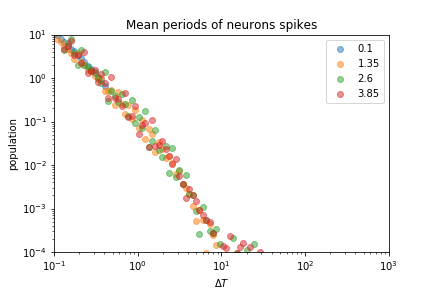
\includegraphics[width = \textwidth]{../papers_studies/figs/IF/mean_spiking_persiods.png}
		\caption{توزیع بسامدی شبکه‌های ۱۰۰۰ نورونی که هر کدام قدرت اتصال متفاوتی دارند. }
		\label{fig:if_isi}
	\end{subfigure}
	\hfill
	\begin{subfigure}[b]{0.5\textwidth}
		\centering
		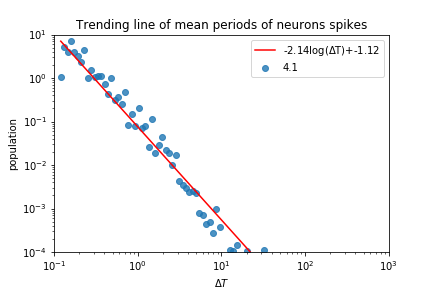
\includegraphics[width = \textwidth]{../papers_studies/figs/IF/mean_spiking_persiods_with_trending_line.png}
		\caption{محاسبه‌ی نمای توزیع توانی فاصله زمانی بین تیزه‌ها}
		\label{fig:if_isi_trending_line}
	\end{subfigure}
	\hfill
	\begin{subfigure}[b]{0.5\textwidth}
		\centering
		\includegraphics[width = \textwidth]{../scripts/all_neurons_model_in_one_place/IF_ensembles/N10000_T1000_I1.2_2.8_cluster_computed/sigma_phase_space_contour.png}
		\caption{صفحه‌ی فاز مربوط به سامانه‌ی نورون‌های انباشت‌وشلیک: پیوست \ref{appendix:phase_sampling_if}}
		\label{fig:if_g_d_phase_space}
	\end{subfigure}
\end{figure}

\زیرقسمت{انحراف از معیار میدان}
مهم‌ترین شاخصه ما برای ردگیری همگامی، انحراف معیار میدان $E$ است که با زیگما $\sigma$ نمایش می‌دهیم. جهش به وجود آمده در شکل‌ (\ref{fig:if_phase_transition}) به این معنی است که سامانه از حالت ناهم‌گامی به هم‌گامی تغییر فاز داده است. 



\زیرقسمت{نورون‌های خاموش}
بی‌تردید میدان داخلی نورون‌ها کاملا تابعی است از آمارتیزه‌های درون سامانه. نورون‌هایی که گاهی برای تیزه زدن به پیش می‌روند و گاه به علت حضور میدان داخلی مهار به عقب برمی‌گردند. خوب است بپرسیم که برآیند این رفت و برگشت‌ برای هر نورون چگونه است. آیا این رفت و برگشت منجر به رسیدن به آستانه‌ی تیزه زدن می‌شود و یا نورون در برآیند اصلا پیشروی نمی‌کند و هیچگاه به آستانه نمی‌رسد و خاموش می‌ماند.\\
در شکل \ref{fig:if_silent_neurons} شمار نورون‌هایی که هیچگاه در سامانه تیزه نمی‌زنند را آورده‌ایم و این که چگونه با با افزایش ضریب تاثیر مهاری میدان این آمار رشد می‌کند.\\
این مشاهده نشان می‌دهد که در فاز هم‌گام، تقریبا ۲۵ درصد نورون‌ها خاموش هستند و نقشی در برقراری جریان داخلی ندارند. قابل حدس است که نورون‌هایی خاموش هستند که جریان‌های تصادفی خارجی پایین دست را داشته‌اند. به این معنی که اگر بازه‌ی جریان تصادفی را تنگ‌تر می‌گرفتیم [ مثلا از$1.6$ ] شروع می‌کردیم؛ سامانه در فاز هم‌گام تفاوت رفتاری نمی‌داشت.\\
همچنین جالب است که تغییر فاز مشاهده شده در تعداد نورون‌های خاموش - شکل \ref{fig:if_silent_neurons}-در حالتی در همسایگی و متمایز از تغییر فاز شکل \ref{fig:if_phase_transition} نشان می‌دهد.


\زیرقسمت{توزیع تناوب زمانی تیزه‌ها}
شبکه‌ی ما متشکل از نورون‌هایی است که مدام در حال تیزه زدن و فعال نگه‌داشتن شبکه هستند. برخی با بسامد بیشتری تیزه می‌زنند و برخی آهسته‌تر. اگر کنجکاو باشیم که جمعیت کل نورون‌های ما چگونه میان دسته‌های مختلف با تناوب‌های متفاوت توزیع شده‌ است؛ لازم است تا توزیع فراوانی آن‌ها را یکجا رسم کنیم - شکل \ref{fig:if_isi}.\\
همان طور که می‌بینید به ظاهر این توزیع رفتاری توانی دارد و اگر کنجکاو باشیم می‌توانیم شیب این نمودار تمام لگاریتمی آن را جهت محاسبه‌ی نمای توزیع بدست آوریم - شکل \ref{fig:if_isi_trending_line}.

\زیرقسمت{پهن‌کردن قالی صفحه‌ی فاز}
در قسمت‌های پیشین تنها به مطالعه‌ی تاثیر ضریب اتصال در تغییرفاز پرداختیم و زمان تاخیر را تنها در $t_d = 0.1 s$ خلاصه کردیم. حال اجازه دهید تا به تاخیر نیز اجازه‌ی تغییر دهیم. در ادامه‌ی این قسمت از نوشتارمان، به فرش‌کردن صفحه‌ی فاز خود خواهیم پرداخت. امید است که چهره‌ی تمام نمای سامانه‌ بر صورت این قالی نقش بندد.\\


\زیرزیرقسمت{قالی انحراف از معیار میدان}
در شکل \ref{fig:if_g_d_phase_space} مشاهده می‌کنیم که شدت هم‌گامی در هر کدام از هنگردهای سامانه چقدر است. این شکل شامل اطلاعات بسیار مفیدی است:

\begin{enumerate}[1.]
	\item 
	به نظر می‌رسد که با افزایش زمان تاخیر و ضریب تاثیر همگامی قدرت پیدا می‌کند
	\item 
	اگر چه تاخیر در جابجایی ضریب‌تاثیر بحرانی تغییری ایجاد نکرده است اما هم‌گامی را قدرت می‌بخشد.
	\item
	اگر ضریب‌تاثیر را بسیار بزرگ کنیم و فاصله‌ی زیادی از ضریب‌تاثیر بحرانی بگیریم؛ شدت هم‌گامی ضعیف می‌شود. این نکته می‌تواند به علت رشد جمعیت نورون‌های خاموش باشد که از تیزه‌زدن محروم می‌شوند و نمی‌توانند خیزهای بلندی را به جریان داخلی القا کنند.
\end{enumerate}

\زیرقسمت{امکانی برای توصیف تحلیلی؟}
برونل در مقاله‌ی خود 
\cite{brunel2000dynamics}
راه‌حلی تحلیلی برای توصیف گذر فاز در مدل انباشت‌وشلیک ارائه کرده است. قصد ما در این جستار تکرار کار برونل نیست اما از راه‌حل برونل الهام خواهیم گرفت تا مدل‌های دیگر نورونی را توصیف و تحلیل کنیم.
